% Created 2020-11-06 fre 15:22
% Intended LaTeX compiler: pdflatex
\documentclass[11pt]{article}
\usepackage[utf8]{inputenc}
\usepackage[T1]{fontenc}
\usepackage{graphicx}
\usepackage{grffile}
\usepackage{longtable}
\usepackage{wrapfig}
\usepackage{rotating}
\usepackage[normalem]{ulem}
\usepackage{amsmath}
\usepackage{textcomp}
\usepackage{amssymb}
\usepackage{capt-of}
\usepackage{hyperref}
\usepackage[english]{babel}
\usepackage[lf]{ebgaramond}
\usepackage{sectsty}
\allsectionsfont{\sf}
\hypersetup{colorlinks=true,linkcolor=black,urlcolor=black}
\usepackage[style=bath,natbib=true,backend=biber,hyperref=false,
doi=false, url=false]{biblatex}
\assignrefcontextentries[]{*}
\bibliography{./biblio_cyrino.bib}
\renewcommand*{\ppspace}{\addspace}
% \DeclareFieldFormat*{parens}{#1\addperiod\addspace}

%% \renewcommand*{\nameyeardelim}{\space}%
%% \renewcommand{\postnotedelim}{: }%
\setcounter{secnumdepth}{0}
\author{Henrik Frisk, henrik.frisk@kmh.se}
\date{\today}
\title{An Exlicapble hunger av Marina Pereira Cyrino}
\hypersetup{
 pdfauthor={Henrik Frisk, henrik.frisk@kmh.se},
 pdftitle={An Exlicapble hunger av Marina Pereira Cyrino},
 pdfkeywords={},
 pdfsubject={},
 pdfcreator={Emacs 26.3 (Org mode 9.4)}, 
 pdflang={English}}
\begin{document}

\maketitle
Marina Pereira Cyrino's avhandling \emph{An Exlicable Hunger: flutist)body(flute (dis)encounters} lades from vid Göteborgs Universitet den 3 april 2019 och opponent var Catherine Laws, pianist och musikvetare baserad vid University of York. Avhandlingen består av en bok och hela tio videor som på olika sätt dokumenterar de fem verk som avhandlingen innefattar. Boken är uppdelad i två delar varav den första fungerar som en slags kappa, en på ett sätt fristående essä, som inte desto mindre ringar in forskningen. Den andra delen diskuterar de konstnärliga verken under rubrikerna: \emph{Nocttuidae, Noctuoidea}, \emph{Is She?}, \emph{An Aeroelastic Flutter}, \emph{Inside-Out Pastoral}, \emph{Check Out My W/holes}.

Metoden i projektet kretsar kring begrepp som transversalitet och "'mixture', 'contamination' and the practice
of 'un-goaling'" \citep[s. 7 (abstract)]{Cyrino2019}. Rollerna som blandas och upplöses är hennes egen "flutist-body-flute" i mötet med andra konstnärers praktik. Metamorfos är ett begrepp som används analytiskt och som präglar avhandlingens första del (men sedan endast förekommer sporadiskt). Referensen är författaren och nobelpristagaren Elias Canetti, och jag tror den är hämtad ur hans föreläsning \emph{The Writers Profession} från 1976 (men här saknas ett direkt citat). Det är diktarens "gift of metamorphosis" som avses och som Cyrino tar avstamp i. En viktig teoretisk referens i texten är också den Brasilianska psykoanalytikern och Guattarilärljungen Suely Rolnik och Cyrino är tydligt inspirerad av poststrukturalistisk teori i allmänhet. Hon vänder sig till Globokars kritik av hyperspecialiseringen i det kapitalistiska samhället och formulerar en mycket skarpt kritik av den europeiska konservatoriemodellen, som jag upplever är hämtad ur en personlig erfarenhet:

\begin{quote}
The ensuing fear, though, simply reinforces the slogan of
"maintaining excellence", of a disciplinary practice, of a certain
kind of virtuosity that rejects everything that is not in direct
accordance with a systematic, intensive and unquestionable
practice, imposed as "tradition", which hinders the opening
toward a diversity of marginal and experimental practices. \citep[s. 23]{Cyrino2019}
\end{quote}

Det är genom denna redogörelse som man kan förstå hur hela hennes projekt har gått mot en praktik som inte längre ser flöjten som en \emph{flöjt}, utan som ligger betydligt närmare ett kompositoriskt arbete där dekonstruktionen av den traditionella flöjten som kulturellt objekt står i centrum. Detta är utan tvekan intressant och ligger ganska nära hur flera andra konstnärliga doktorandprojekt har utvecklat sin praktik. Som nämnts är hela avhandlingen är situerad i poststrukturalistisk, och även postkolonial och feministisk teori, med intressanta referenser som Ellen Watermans analys av Brian Ferneyhoughs \emph{Cassandra's Dream Song} \citep{Waterman1994}, som i sin tur relaterar till \emph{Cass\ldots{}andra} (se kapitlet \emph{Is She?} i avhandlingen), ett verk som kan ses som en slags fri nytolkning och gestaltning av Ferneyhoughs klassiska soloflöjtverk.

Den andra delen diskuterar som sagt de konstnärliga arbetena, varav flera är dokumenterade som videoessäer. Det formatet är intressant och bidrar till en upplevd närhet till det konstnärliga arbetet. Kapitlena har ganska olika karaktär och stilen i skrivandet varierar mellan ett poetiskt lekande med ord och former (cirklar av ord eller teckningar av ord), och ett filosofiskt orienterat och mer akademiskt skrivande. Tillsammans med videoessäernas poetiska bild- och ljudspråk blir helheten, trots de stora stilistiska variationerna, ändå sammanhållen.

I det andra kapitlet i den andra delen, \emph{Is She?}, diskuterar Cyrino arbetet med tidigare nämnda \emph{Cass\ldots{}andra} (Mansoor Hosseinis, 2015), ett verk jag har sett henne framföra live.\footnote{\emph{Sett}, snarare än hört då detta är ett minst lika mycket visuellt performanceverk som ett framförande av en komposition. Framförandet ägde rum på Artisten i Göteborg i samband med ett delseminarium.} Videoessän, med samma namn som kapitlet, \emph{Is She?}, är en gestaltning, snarare än en inspelning av \emph{Cass\ldots{}andra}, då den lägger till information till liveversionen. Bara perspektivförflyttningen som videoformatet erbjuder gör upplevelsen till något helt annorlunda. Nackdelen med konstnärliga dokumentationer av det här slaget är egentligen samma som fördelen: att formatet lägger till information och estetiserar själva formen för dokumentationen. Resultatet blir således mer än en ren dokumentation av framförandet -- vilket för övrigt är en omöjlighet. Istället framträder videon som ett konstnärligt uttryck i sig självt, och därmed är det egentligen inte heller en videoessä, utan snarare ett videoverk. Men jag återkommer till det senare.

Om avhandlingen fram till nu har fortsatt i det spår som den öppnade i, med en kritik av den klassiska musikens hierarkier och dominanta strukturer, så börjar den i tredje kapitlet en i och för säg följdriktig resa bort från just musiken. Ett nytt och ännu mer poetiskt språk med intertextuella referenser tillbaka till föregående kapitel i avhandlingen ger vid handen en text som inte beskriver en process, utan som \emph{är} en process. Min tolkning är att detta är ett försök att visa att avhandlingen inte är en samling självständiga verk, utan ett där processen står i centrum och verken är avknoppningar av denna. Initialt i tredje kapitlet ställs en fråga som jag ser som ett försök att rama in fältet:

\begin{quote}
How to speak out of the exotification of bewitching flutes, of
bewitching prophetesses, of bewitching female bodies? As a
possible answer, An Aeroelastic Flutter spins around the tragic
female voice, searching for ways to work around/ detour/
dribble the female body as a place of curse and punishment. \citep[s. 80]{Cyrino2019}
\end{quote}
Resten av kapitlet ringar bokstavligt talat in citat från historiska texter, Gertrude Stein och populärkulturella referenser, liknande det i bilden (se \ref{cyrino1}).

\label{cyrino1}
\begin{figure}[htbp]
\centering
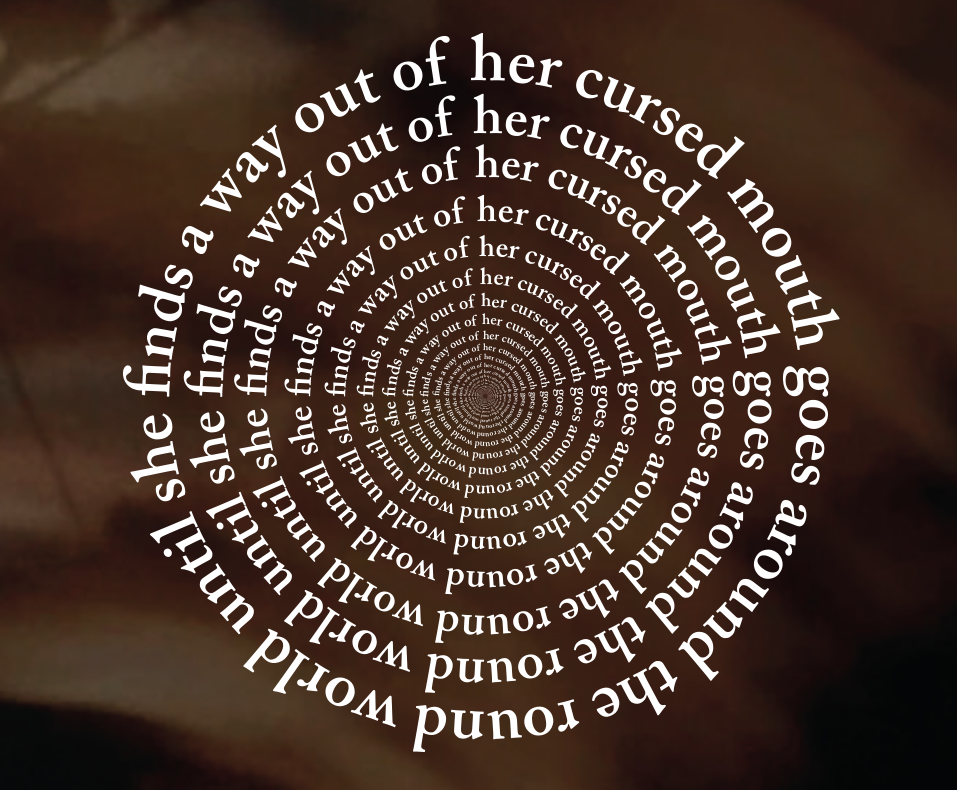
\includegraphics[width=.9\linewidth]{images/2020-11-03_20-04-54_screenshot.png}
\caption{Del av sid 118 från Cyrino, M. P., An exlicable hunger. Texten i cirkeln är hämtad från texten till  \emph{Francisco, el hombre. Triste louca ou má}, ett spår från skivan SOLTASBRUXA (2016).}
\end{figure}

Ett viktigt fokus för Cyrino i avhandlingen är konstnärliga samarbeten. Så gott som alla verk i avhandlingen är samarbeten med andra konstnärer från olika discipliner, och detta ska ses som en styrka. Hon benämner det som "co-creation" som skulle kunna översättas till sam-skapande. I hennes fall ska det ses som ambitionen att genom att arbeta kreativt \emph{med} en annan konstnär så ges hon möjligheten att upptäcka nya sidor av sitt eget skapande. Det fjärde kapitlet, \emph{Inside-Out Pastoral}, är en beskrivning av ett sådant sam-skapande med den brasilianska bildkonstnären Marina Nazareth. Texten är delvis handskriven och följer de böljande vågor som utgör konstnärens teckningar. I det avslutande kapitlet knyter texten an till där den började.

Frågan som jag menar behöver ställas, och som jag antydde tidigare i texten, är vad som är vunnet på att gestalta dokumentation som en egen konstnärlig genre och text som en konstform i sig. Även om jag är delvis kritisk till utfallet i den här avhandlingen, betyder det inte att det inte bör experimenteras med. Dokumentation är inte en egen genre, men om det finns en möjlighet att kommunicera konstnärlig praktik och dess processer genom att gestalta dokumentation som ett uttryck i sig själv så ska det naturligtvis göras. Om det görs, och det menar jag att Cyrino försöker göra, så uppstår minst en avgörande fråga: hur bedöms kvaliteten om musiken är inbäddad i ett arteget metaformat? I en konstnärligt gestaltad videoessä som \emph{My Inside-out Pastoral} blir det precis som med \emph{Is She?} svårt att inte se den som ett viedoverk snarare än en essä eller ett musikframförande. Hur ska den i så fall kontextualiseras för att gestaltningen ska kunna förstås?

Under sommaren 2020 pågick en debatt om konstnärlig forskning som uppstod som en följd av en underkänd avhandling vid Stockholms Konstnärliga högskola.\footnote{Se högskolans hemsida för mer information: \url{https://www.uniarts.se/forskning-utvecklingsarbete/doktorandprojekt/fauxthentication} (besökt den 30 oktober, 2020)} Det underkända doktorandprojektet berör huruvida konst producerad som konstnärlig forskning överhuvudtaget kan betraktas som det som bildkonsten brukar beteckna som fri konst. Att fri konst är själva \emph{ämnet} för såväl grundutbildningar som forskarutbildningar på t.ex. Göteborgs Universitet har mindre betydelse här. Påståendet som gödde debatten var den att konstnärlig forskning akademiserar konsten på ett sätt som enligt vissa förstör just den fria konsten \citep[se till exempel ][]{petersson2020}. Jag skulle vilja hävda att \emph{An Explicable Hunger} är ett bevis på att även konstnärlig forskning är fri i någon mån och därmed blir avhandlingen ett levande exempel på hur oinitierad diskussionen har varit. En flöjtist som gör en avhandling som ligger närmare performancekonst än flöjtinterpretation är i sig ett exempel på att formaliserade bedömningsmatriser som tvingar in konsten i på förhand bestämda fack åtminstone inte dominerar Göteborgs universitet. Intensiteten i kritiken, som egentligen inte går att bemöta såsom den framställdes, gör ändå att den uppföljande frågan kan bli problematisk, men den behöver ändå ställas: vad är själva kärnan i ett konstnärligt forskningsarbete? Det konstnärliga uttrycket som metod i allmänhet, eller är det den specifika disciplinens förutsättningar i synnerhet? Eller är kan den, som i Cyrinos arbete, röra sig från det ena till det andra?

Sedan konstnärlig forskning etablerade sig i Sverige har det funnits
en idé om att den övergripande metoden som utgår från konstnärlig
praktik förenar alla konstnärliga discipliner. Även om det var ett
produktivt tillvägagångssätt i ett tidigt skede vill jag hövda att det
nu är viktigt att låta de olika disciplinerna utveckla sina egna
metoder. Att fri konst och musik har den konstnärliga metoden gemensam
betyder inte att de som forskningsdiscipliner har mer gemensamt än,
säg, pedagogik och kärnfysik, som delar den vetenskapliga metoden. Mot
den bakgrunden kan frågan ställas hur den typ av innehållsmäsig
glidning som vi ser i Cyrinos avhandling kan betraktas. Den är på
inget sätt ovanlig, tvärtom förekommer den allt oftare ofta i nutida
musik \citep{groth2016}. Det
kan diskuteras om Cyrinos videoessäer är en expansion av musikfältet
eller ett steg över i en helt annan disciplin? Det är svårt att svara
på utifrån avhandlingen, men det är som expansion av musikfältet som
jag finner arbetet mest intressant.

\section*{Bibliography}
\label{sec:org2ad5f4c}
\printbibliography
\end{document}